

\chapter{Satellite Communications}



\section{Orbits}\label{2.1}
One crucial topic that anyone working with satellites needs to understand is orbits and their characteristics. An orbit is the \textbf{gravitationally curved path of an object around a center of mass}. Examples of orbits can be the Earth around the Sun or artificial satellites around the Earth.

This section will cover the elements that describe and define an orbit, how it is represented on a map and in which way the elements that define a particular orbit can be delivered so they can be used by a computer.


\subsection{Kepler's Laws}\label{2.1}
Planetary movements were first mathematically defined by the German mathematician, astronomer and astrologer Johannes Kepler in the 17th century. He concentrated his observations into three simple laws\citep{SSEng}:
\begin{itemize}

\item The orbit of each planet is an ellipse with the Sun occupying one focus.
\item The line joining the Sun to a planet sweeps out equal areas in equal intervals of time.
\item A planet's orbital period is proportional to the mean distance between the Sun and the planet, raised to the power of 3/2.
\end{itemize} 

These laws apply to every celestial body. When analysing to bodies, if one is much bigger than the other, it conforms the "two-body problem". It assumes that both bodies are spherical and they are modelled as if they were point particles. This means that influences from any third body are discarded. The analysis of hits problem has resulted in six elements that completely define an orbit, which will be explained in the next section.


\pagebreak
\subsection{Classical Orbital Elements}\label{2.2}
The Classical Orbital Elements are six parameters which uniquely identify an orbit. They also can be used to predict future positions of the satellite.\cite{IntAstr}

The first two elements, the orbit's size and shape are defined based on a 2D representation on an ellipse (Figure \ref{f2.1}).

\begin{figure}[H]
\centerline{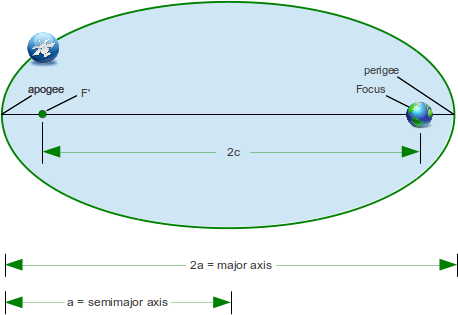
\includegraphics[width=0.7\textwidth]{images/Ellipse.png}}
\caption{Semimajor Axis}
\label{f2.1}
\end{figure}

\begin{itemize}
\item The \emph{semimajor axis} ($a$) is one half the distance across the long axis of the orbit, and it represents the orbit's size.
\item The \emph{eccentricity} represents the shape of the orbit. It describes how much the ellipse is elongated compared to a circle. Based on the latter, the orbit can have the following shapes, as shown in Figure \ref{f2.2}

\begin{figure}[H]
\centerline{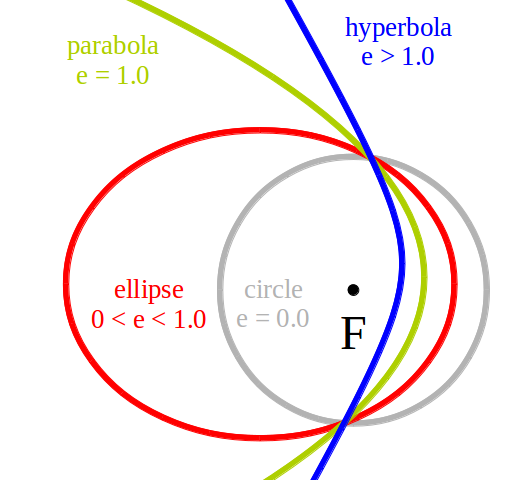
\includegraphics[scale=0.35]{images/Eccentricity.png}}
\caption{Eccentricity}
\label{f2.2}
\end{figure}

\end{itemize}


Before jumping onto the next Orbital Elements it is necessary to point out that the Geocentric-equatorial Coordinate System will be used. It is now a 3D representation, where the fundamental plane is Earth's equatorial plane and the principal direction is in the vernal equinox direction.

The following orbital elements define the orientation of the orbital plane:

\begin{itemize}
\item The inclination ($i$) describes the tilt of the orbital plane with respect to the reference plane. It is measured at the ascending node. This is, where the orbit crosses with the reference plain when moving upwards.
\item The right ascension of the ascending node ($\Omega$) represents the angle between the principal direction and the point where the orbital plane crosses the reference plane from south to north measured eastward. 
\end{itemize}

Based on this two elements, the orbits can be classified as shown in Table \ref{Table2.1}

\begin{table}[h]
\centering
\begin{tabular}{|c|c|c|}
\hline
\begin{tabular}[x]{@{}c@{}}\textbf{Inclination ($i$)}\end{tabular} &
\begin{tabular}[x]{@{}c@{}}\textbf{Orbital Type}\end{tabular} &
\begin{tabular}[x]{@{}c@{}}\textbf{Diagram}\end{tabular}\\
\hline
\begin{tabular}[x]{@{}c@{}} 0$^\circ$ or 180$^\circ$\end{tabular} &
\begin{tabular}[x]{@{}c@{}}Equatorial\end{tabular} &
\begin{tabular}[x]{@{}c@{}}\raisebox{-\totalheight}{
\includegraphics[scale=0.5]{images/EquatorialOrbit.png}}\end{tabular}\\
\hline
\begin{tabular}[x]{@{}c@{}} 90$^\circ$\end{tabular} &
\begin{tabular}[x]{@{}c@{}}Polar\end{tabular} &
\begin{tabular}[x]{@{}c@{}}\raisebox{-\totalheight}{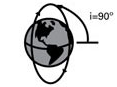
\includegraphics[scale=0.5]{images/PolarOrbit.png}}\end{tabular}\\
\hline
\begin{tabular}[x]{@{}c@{}} 0$^\circ$ $\leq$ $i$ $<$ 90$^\circ$\end{tabular} &
\begin{tabular}[x]{@{}c@{}}Direct or Prograde (moves in the\\ direction of Earth's rotation)\end{tabular} &
\begin{tabular}[x]{@{}c@{}}\raisebox{-\totalheight}{
\includegraphics[scale=0.5]{images/DirectOrbit.png}}\end{tabular}\\
\hline
\begin{tabular}[x]{@{}c@{}} 90$^\circ$ $<$ $i$ $\leq$ 180$^\circ$\end{tabular} &
\begin{tabular}[x]{@{}c@{}}Indirect or Retrograde (moves against\\ the direction of Earth's rotation)\end{tabular} &
\begin{tabular}[x]{@{}c@{}}\raisebox{-\totalheight}{
\includegraphics[scale=0.5]{images/IndirectOrbit.png}}\end{tabular}\\
\hline
\end{tabular}
 \caption{Types of Orbits and Their Inclination \cite{IntAstr}.}
  \label{Table2.1}
\end{table}


Although it is not part of the COEs, orbits can also be sorted by their altitude. NASA's classification divides orbits in three groups (Table \ref{Table2.2}).

\begin{table}[h]
\centering
\begin{tabular}{|c|c|c|}
\hline
\begin{tabular}[x]{@{}c@{}}\textbf{Orbit}\end{tabular} &
\begin{tabular}[x]{@{}c@{}}\textbf{Altitude ($a$)}\end{tabular} &
\begin{tabular}[x]{@{}c@{}}\textbf{Uses}\end{tabular}\\
\hline
\begin{tabular}[x]{@{}c@{}}Low Earth Orbit (LEO)\end{tabular} &
\begin{tabular}[x]{@{}c@{}}$a < 2000 Km$\end{tabular} &
\begin{tabular}[x]{@{}c@{}}Scientific and weather\\ satellites
\end{tabular}\\
\hline
\begin{tabular}[x]{@{}c@{}}Medium Earth Orbit (MEO)\end{tabular} &
\begin{tabular}[x]{@{}c@{}}$2000 Km \leq a < 36000 Km$\end{tabular} &
\begin{tabular}[x]{@{}c@{}}GPS\end{tabular}\\
\hline
\begin{tabular}[x]{@{}c@{}}High Earth Orbit (HEO) or \\
Geosynchronous (GSO)\end{tabular} &
\begin{tabular}[x]{@{}c@{}}$36000 Km$\end{tabular} &
\begin{tabular}[x]{@{}c@{}}Communications\\(phones, television,\\ radio)
\end{tabular}\\
\hline
\end{tabular}
 \caption{NASA's classification of orbits. \cite{NASAOrbits}}
  \label{Table2.2}
\end{table}
\pagebreak

It is now time to go through the last two COEs:
\begin{itemize}
\item The argument of perigee ($\omega$) is the angle between the ascending node and the perigee, measured in the direction of the satellite's motion.
\item The true anomaly ($\upsilon$) specifies the location of the satellite within the orbit. Amongst all the CEOs, this is te only one which changes over time. It is the angle between the perigee and the satellite's position vector measured in the direction of its motion.
\end{itemize}

\begin{figure}[H]
\centerline{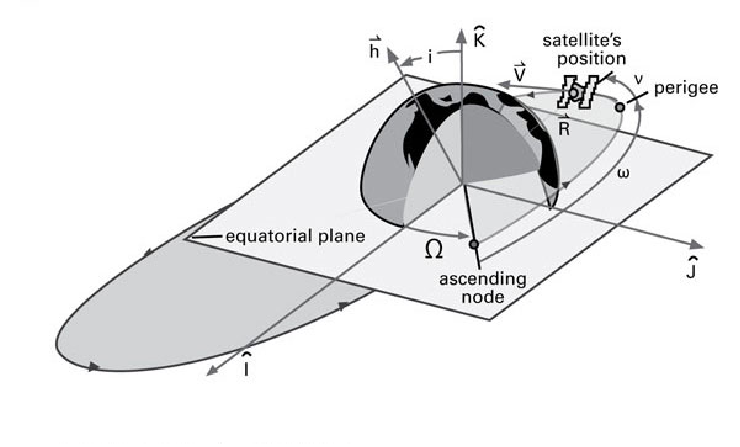
\includegraphics[width=0.7\textwidth]{images/COEs.png}}
\caption{Classical Orbital Elements \cite{IntAstr}}
\label{f2.3}
\end{figure}
\pagebreak
\subsection{Ground Tracks}\label{2.3}

The satellite ground tracks are the projection of its orbit onto Earth. An example of this can be Figure \ref{f2.4}.

\begin{figure}[H]
\centerline{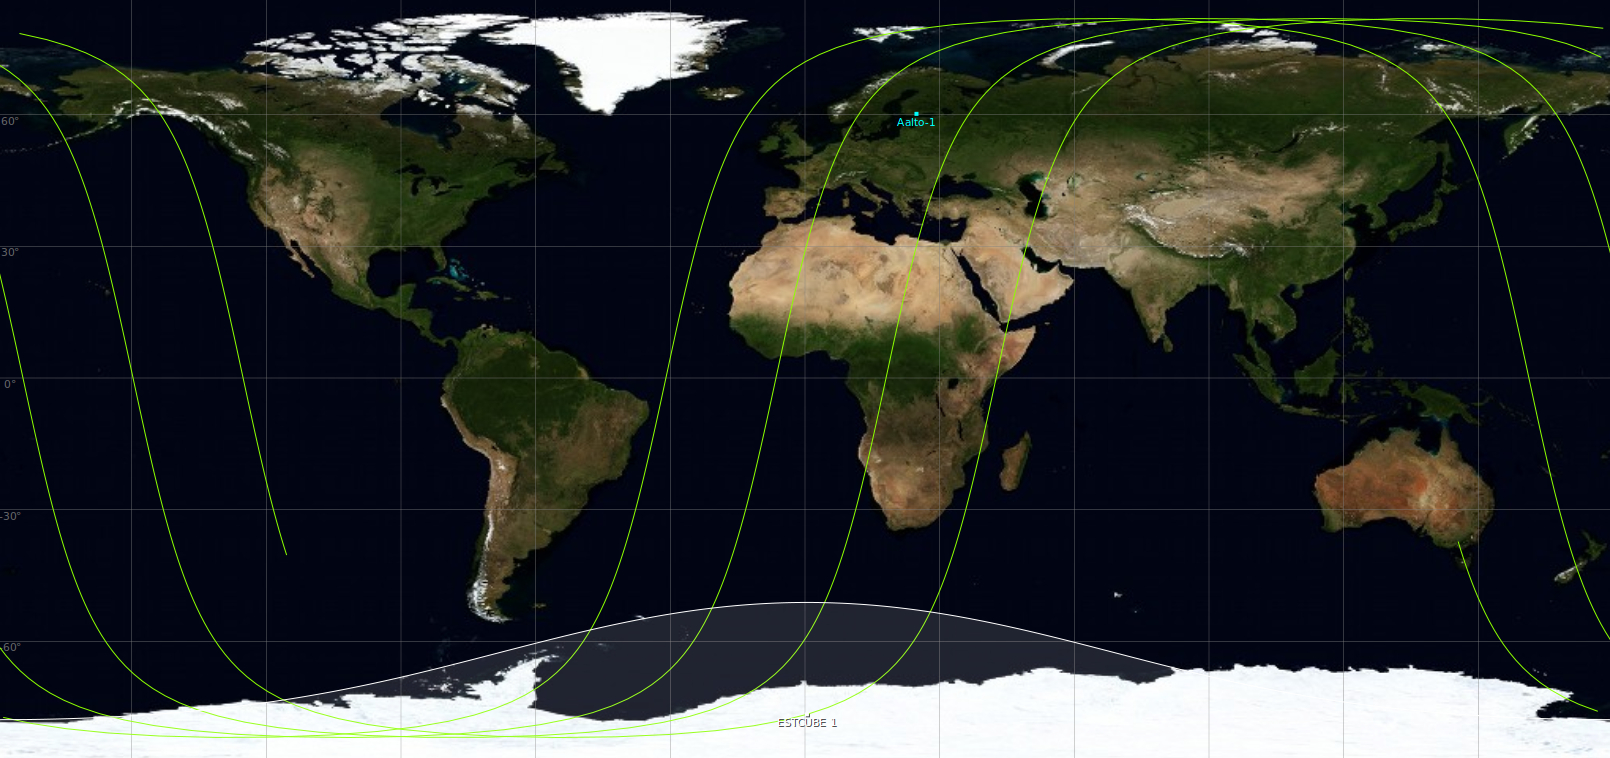
\includegraphics[width=1\textwidth]{images/GroundTracks.png}}
\caption{Ground Tracks of ESTCube-1}
\label{f2.4}
\end{figure}

Since the orbital plane does not move in inertial space, the satellite's orbit will always be the same. If Earth did not move the representation of the orbit would be a single line, as the ground track would continuously repeat. However, Earth rotates at 1600 km/hr. Thus, even if the orbit does not change, from the Earth-based observer's point of view it appears to shift to the west.

\subsection{Two Line Elements}\label{2.4}
A two line element set (TLE) is a data format created by the North American Aerospace Defense Command (NORAD) and NASA to transport sets of orbital elements describing satellite orbits around Earth. These TLEs can be later processed by a computer to calculate the position of a satellite at a particular time.
\newpage
The following snippet shows an example of a TLE for the International Space Station.

\noindent \texttt{\footnotesize ISS (ZARYA)\newline
1 25544U 98067A   13166.62319444  .00005748  00000-0  10556-3 0   120\newline
2 25544  51.6483 116.0964 0010829  73.3727 265.7013 15.50799671834453}\\

\begin{table}[h]
\centering
\begin{tabular}{|l|l|l|l|}
\hline
\begin{tabular}[x]{@{}c@{}}\textbf{Field}\end{tabular} &
\begin{tabular}[x]{@{}c@{}}\textbf{Columns}\end{tabular} &
\begin{tabular}[x]{@{}c@{}}\textbf{Content}\end{tabular} &
\begin{tabular}[x]{@{}c@{}}\textbf{Example}\end{tabular}\\
\hline
\begin{tabular}[x]{@{}c@{}}1\end{tabular} &
\begin{tabular}[x]{@{}c@{}}01\end{tabular} &
\begin{tabular}[x]{@{}c@{}}Line number\end{tabular} &
\begin{tabular}[x]{@{}c@{}}1\end{tabular}\\
\hline
\begin{tabular}[x]{@{}c@{}}2\end{tabular} &
\begin{tabular}[x]{@{}c@{}}03-07\end{tabular} &
\begin{tabular}[x]{@{}c@{}}Satellite number\end{tabular} &
\begin{tabular}[x]{@{}c@{}}25544\end{tabular}\\
\hline
\begin{tabular}[x]{@{}c@{}}3\end{tabular} &
\begin{tabular}[x]{@{}c@{}}08\end{tabular} &
\begin{tabular}[x]{@{}c@{}}Classification (U=Unclassified)\end{tabular} &
\begin{tabular}[x]{@{}c@{}}U\end{tabular}\\
\hline
\begin{tabular}[x]{@{}c@{}}4\end{tabular} &
\begin{tabular}[x]{@{}c@{}}10-11\end{tabular} &
\begin{tabular}[x]{@{}l@{}}International Designator\\(Last two digits of launch year)\end{tabular} &
\begin{tabular}[x]{@{}c@{}}98\end{tabular}\\
\hline
\begin{tabular}[x]{@{}c@{}}5\end{tabular} &
\begin{tabular}[x]{@{}c@{}}12-14\end{tabular} &
\begin{tabular}[x]{@{}l@{}}International Designator\\ (Launch number of the year)\end{tabular} &
\begin{tabular}[x]{@{}c@{}}067\end{tabular}\\
\hline
\begin{tabular}[x]{@{}c@{}}6\end{tabular} &
\begin{tabular}[x]{@{}c@{}}15-17\end{tabular} &
\begin{tabular}[x]{@{}c@{}}International Designator (Piece of the launch)\end{tabular} &
\begin{tabular}[x]{@{}c@{}}A\end{tabular}\\
\hline
\begin{tabular}[x]{@{}c@{}}7\end{tabular} &
\begin{tabular}[x]{@{}c@{}}19-20\end{tabular} &
\begin{tabular}[x]{@{}l@{}}Epoch Year (Last two digits of year)\end{tabular} &
\begin{tabular}[x]{@{}c@{}}08\end{tabular}\\
\hline
\begin{tabular}[x]{@{}c@{}}8\end{tabular} &
\begin{tabular}[x]{@{}c@{}}21-32\end{tabular} &
\begin{tabular}[x]{@{}l@{}}Epoch (Day of the year and fractional\\portion of the day)\end{tabular} &
\begin{tabular}[x]{@{}c@{}}264.51782528\end{tabular}\\
\hline
\begin{tabular}[x]{@{}c@{}}9\end{tabular} &
\begin{tabular}[x]{@{}c@{}}34-43\end{tabular} &
\begin{tabular}[x]{@{}c@{}}First Time Derivative of the Mean Motion\end{tabular} &
\begin{tabular}[x]{@{}c@{}}-0.00002182\end{tabular}\\
\hline
\begin{tabular}[x]{@{}c@{}}10\end{tabular} &
\begin{tabular}[x]{@{}c@{}}45-52\end{tabular} &
\begin{tabular}[x]{@{}l@{}}Second Time Derivative of Mean Motion\\(decimal point assumed)\end{tabular} &
\begin{tabular}[x]{@{}c@{}}00000-0\end{tabular}\\
\hline
\begin{tabular}[x]{@{}c@{}}11\end{tabular} &
\begin{tabular}[x]{@{}c@{}}54-61\end{tabular} &
\begin{tabular}[x]{@{}c@{}}BSTAR drag term (decimal point assumed)\end{tabular} &
\begin{tabular}[x]{@{}c@{}}-11606-4\end{tabular}\\
\hline
\begin{tabular}[x]{@{}c@{}}12\end{tabular} &
\begin{tabular}[x]{@{}c@{}}63\end{tabular} &
\begin{tabular}[x]{@{}c@{}}Ephemeris type\end{tabular} &
\begin{tabular}[x]{@{}c@{}}0\end{tabular}\\
\hline
\begin{tabular}[x]{@{}c@{}}13\end{tabular} &
\begin{tabular}[x]{@{}c@{}}65-68\end{tabular} &
\begin{tabular}[x]{@{}c@{}}Element number\end{tabular} &
\begin{tabular}[x]{@{}c@{}}292\end{tabular}\\
\hline
\begin{tabular}[x]{@{}c@{}}14\end{tabular} &
\begin{tabular}[x]{@{}c@{}}69\end{tabular} &
\begin{tabular}[x]{@{}l@{}}Checksum (Modulo 10)\\(Letters, blanks, periods, plus signs = 0;\\minus signs = 1)\end{tabular} &
\begin{tabular}[x]{@{}c@{}}7\end{tabular}\\
\hline
\end{tabular}
 \caption{Two-Line Element Set Format Definition, Line 1} 
  \label{Table2.3}
\end{table}
\pagebreak

\begin{table}[h]
\centering
\begin{tabular}{|l|l|l|l|}
\hline
\begin{tabular}[x]{@{}c@{}}\textbf{Field}\end{tabular} &
\begin{tabular}[x]{@{}c@{}}\textbf{Columns}\end{tabular} &
\begin{tabular}[x]{@{}c@{}}\textbf{Content}\end{tabular} &
\begin{tabular}[x]{@{}c@{}}\textbf{Example}\end{tabular}\\
\hline
\begin{tabular}[x]{@{}c@{}}1\end{tabular} &
\begin{tabular}[x]{@{}c@{}}01\end{tabular} &
\begin{tabular}[x]{@{}c@{}}Line number\end{tabular} &
\begin{tabular}[x]{@{}c@{}}1\end{tabular}\\
\hline
\begin{tabular}[x]{@{}c@{}}2\end{tabular} &
\begin{tabular}[x]{@{}c@{}}03-07\end{tabular} &
\begin{tabular}[x]{@{}c@{}}Satellite number\end{tabular} &
\begin{tabular}[x]{@{}c@{}}25544\end{tabular}\\
\hline
\begin{tabular}[x]{@{}c@{}}3\end{tabular} &
\begin{tabular}[x]{@{}c@{}}09-16\end{tabular} &
\begin{tabular}[x]{@{}c@{}}Inclination [Degrees]\end{tabular} &
\begin{tabular}[x]{@{}c@{}}51.6416\end{tabular}\\
\hline
\begin{tabular}[x]{@{}c@{}}4\end{tabular} &
\begin{tabular}[x]{@{}c@{}}18-25\end{tabular} &
\begin{tabular}[x]{@{}l@{}}Right Ascension of the Ascending\\Node [Degrees]\end{tabular} &
\begin{tabular}[x]{@{}c@{}}247.4627\end{tabular}\\
\hline
\begin{tabular}[x]{@{}c@{}}5\end{tabular} &
\begin{tabular}[x]{@{}c@{}}27-33\end{tabular} &
\begin{tabular}[x]{@{}l@{}}Eccentricity (decimal point assumed)\\ (Launch number of the year)\end{tabular} &
\begin{tabular}[x]{@{}c@{}}0006703\end{tabular}\\
\hline
\begin{tabular}[x]{@{}c@{}}6\end{tabular} &
\begin{tabular}[x]{@{}c@{}}35-42\end{tabular} &
\begin{tabular}[x]{@{}c@{}}Argument of Perigee [Degrees]\end{tabular} &
\begin{tabular}[x]{@{}c@{}}130.5360\end{tabular}\\
\hline
\begin{tabular}[x]{@{}c@{}}7\end{tabular} &
\begin{tabular}[x]{@{}c@{}}44-51\end{tabular} &
\begin{tabular}[x]{@{}l@{}}Mean Anomaly [Degrees]\end{tabular} &
\begin{tabular}[x]{@{}c@{}}325.0288\end{tabular}\\
\hline
\begin{tabular}[x]{@{}c@{}}8\end{tabular} &
\begin{tabular}[x]{@{}c@{}}53-63\end{tabular} &
\begin{tabular}[x]{@{}l@{}}Mean Motion [Revs per day]\end{tabular} &
\begin{tabular}[x]{@{}c@{}}15.72125391\end{tabular}\\
\hline
\begin{tabular}[x]{@{}c@{}}9\end{tabular} &
\begin{tabular}[x]{@{}c@{}}64-68\end{tabular} &
\begin{tabular}[x]{@{}c@{}}Revolution number at epoch [Revs]\end{tabular} &
\begin{tabular}[x]{@{}c@{}}56353\end{tabular}\\
\hline
\begin{tabular}[x]{@{}c@{}}10\end{tabular} &
\begin{tabular}[x]{@{}c@{}}69\end{tabular} &
\begin{tabular}[x]{@{}l@{}}Checksum (Modulo 10)\end{tabular} &
\begin{tabular}[x]{@{}c@{}}00000-0\end{tabular}\\
\hline
\end{tabular}
 \caption{Two-Line Element Set Format Definition, Line 2} 
  \label{Table2.4}
\end{table}





\section{Data}
The data exchanged between a satellite and the ground stations on Earth can be divided into three different categories: the beacon, the telemetry and the telecommands.

\subsection{Beacon}

A \emph{beacon} is a radio signal transmitted continuously or periodically over a specified radio frequency. It provides a small amount of information such as identification or location, but it can have more applications. Examples of these are: adjust the power of the ground station signal based on the beacon's strength or tune the ground station to compensate the doppler shift.

\subsection{Telemetry}

\emph{Telemetry} data is sent from the satellite to the ground station and can also be divided in three sub-categories.\\

The \emph{housekeeping data} provides information abouth the health and operating status of the satellite. Examples of this data can be pressure, voltages and currents, or also bits representing the operational status of all the components as it is shown in Figure \ref{f3.1}. The size of this data is usually quite small, so a bit rate on only a few hundres of bits per second is enough to complete the transmission successfully.

\begin{figure}[H]
\centerline{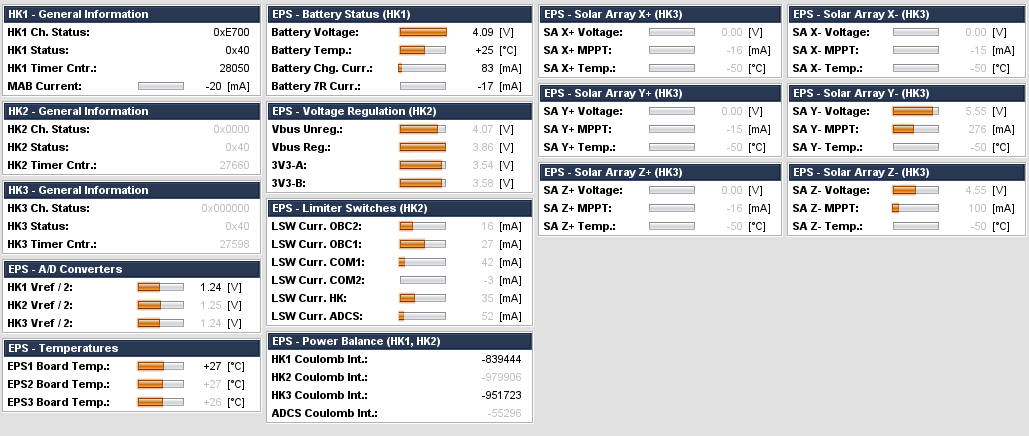
\includegraphics[width=1\textwidth]{images/housekeeping.png}}
\caption{Housekeeping data of the satellite Masat-1}
\label{f3.1}
\end{figure}

\emph{Attitude data} is generated by different sensors, such as magnetometers, gyroscopes, accelerometers and Sun, Earth and star sensors.\\

\emph{Payload data} changes with every mission and needs to be considered individually. Scientific or Earth-observing mission normally generate very large data volumes, specially in the form of images. An example of this can be Figure \ref{f3.2}, the first picture taken by the Hungarian nanosatellite Masat-1\cite{Masat}.

\begin{figure}[H]
\centerline{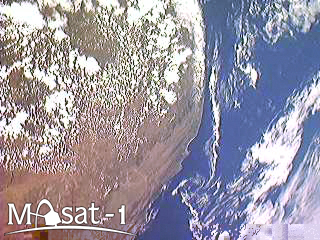
\includegraphics[width=0.7\textwidth]{images/masat.jpg}}
\caption{Picture of South Africa taken from the nanosatellite Masat-1}
\label{f3.2}
\end{figure}
\pagebreak

\subsection{Telecomands}
The telecommands are sent from the ground station to the satellite. They are used to remotely control its functions and are divided in three basic types \cite{SSEng}:
\begin{itemize}
\item \emph{Low-level on-off commands}. These are logic-level pulses used to set or reset log flip-flops.
\item \emph{High-level on-off commands}. Higher-powered pulses, capable of operating a latching relay or RF waveguide switch direcly.
\item \emph{Proportional commands}. Digital words. Used for purposes such as reprogramming memory locations on the on-board computer or setting up registers in the attitude control subsystem.

\end{itemize}

\section{Ground Station}
One integral part of every satellite mission is the ground station. It works as the first and final piece of the communication link. Its main functions are the following:
\begin{itemize}
\item Tracking the satellite to determine its position in orbit.
\item Gather data to keep track of the satellite's data and status.
\item Command operations to control the different functions of the satellite.
\item Process the received engineering and scientific data to present it in the required formats.
\end{itemize}

It is important to remember that university satellites are usually classified as amateur satellites. This means that they use amateur radio frequencies and the usage of the ground station is bound to each country's amateur radio regulations.

\subsection{Hardware}

The main components of a ground station are the antenna, the transceiver, the data recorders and the computers and their peripherals.
\pagebreak
\subsubsection{Antennas}
The main hardware component of a ground station is the antenna. Its functions may include tracking, receiving telemetry, sending telecommands, etc.
\pagebreak

The frequencies most commonly used for amateur satellites are shown in Table \ref{Table3.1}.

\begin{table}[h]

\caption{TODO: Table with Frequencies.}
  \label{Table3.1}
\end{table}
\subsubsection{Transceiver}
A transceiver is a hardware unit containing both a transmitter and a receiver. It acts as an intermediary between the antenna and a computer, changing the radio frequency into bytes and viceversa.

\subsection{Software}
The activity in the ground station does not start when the satellite is passing over it and does not end once it is gone. There are certain tasks that need to be done before, during and after the pass.\\

Before the satellite arrives it is necessary to determine and predict its orbit. Based on this prediction the software will schedule future passes and generate the command list which will be sent during the pass.\\

The real-time software comes into operation when the satellite is visible from the ground station. It is in charge of controlling the antenna rotor to follow it across the sky; it will also send telecommands to the satellite and verify their correct reception. In addition, it will receive the data being transmitted from the satellite, which will be processed later.\\

Once the satellite is not visible any more the post-pass software comes into play. The data received during the pass is now processed and stored so the specialists can analyse it.

\subsection{Protocols}
A protocol is an agreement between the communicating parties on how communication is to proceed\cite{Tanenbaum}. This section will be focused on the OSI Reference model as well as on some of the most popular protocols for amateur radio communications.
\pagebreak
\subsubsection{The OSI Reference Model}
The Open Systems Interconnection (OSI) Reference Model was developed in 1983 and revised in 1995. This model deals with connecting systems that are open for communication with other systems. It consists on seven layers which are explained in Table 3.2.\\

\begin{table}[h]
\centering
\begin{tabular}{|l|l|l|l|}
\hline
\multicolumn{4}{|c|}{\textbf{OSI Model}}\\
\hline\pagebreak
& \textbf{Data Unit} & \textbf{Layer} & \textbf{Function}\\
\hline
\multirow{4}{*}{Host Layers} & \multirow{3}{*}{Data} & 7. Application & Network process to application.\\
\cline{3-4}
& & 6. Presentation & \begin{tabular}[x]{@{}l@{}}Data representation, encryption\\and decryption, convert machine\\dependent data to machine\\independent data\end{tabular}\\
\cline{3-4}
& & 5. Session &\begin{tabular}[x]{@{}l@{}}Interhost communication,\\managing sessions between\\applications\end{tabular}\\
\cline{2-4}
& Segments & 4. Transport & \begin{tabular}[x]{@{}l@{}}End-to-end connection,\\reliability and flow control\end{tabular}\\
\hline
\multirow{3}{*}{Media Layers} & Packet/Datagram & 3. Network & \begin{tabular}[x]{@{}l@{}}Path determination and\\logical adressing\end{tabular}\\
\cline{2-4}
& Frame & 2. Data link & Physical addressing\\
\cline{2-4}
& Bit & 1.Physical & \begin{tabular}[x]{@{}l@{}}Media, signal and\\binary transmission\end{tabular}\\
\hline
\end{tabular}
\caption{OSI Model\cite{Tanenbaum}.}
  \label{Table3.2}
\end{table}

\pagebreak

\subsubsection{AX.25}
AX.25 is a data link layer protocol designed for use by amateur radio operators. It occupies the first, second and third layers of the OSI model. However, AX.25 was developed before the model came into action, so its specification was no written to separate into OSI layers.\\

The link-layer packet radio transmission takes place in small blocks of data called frames. Those frames are represented in the Figures \ref{f3.3} and \ref{f3.4}.\\

 \begin{figure}[H]
\centerline{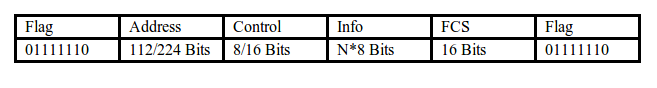
\includegraphics[width=1\textwidth]{images/ax25a.png}}
\caption{Supervisory and Unnumbered frames \cite{AX25}}
\label{f3.3}
\end{figure}

\begin{figure}[H]
\centerline{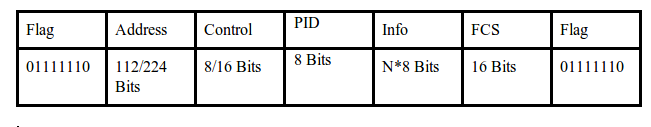
\includegraphics[width=1\textwidth]{images/ax25b.png}}
\caption{AX.25 Information frame \cite{AX25}}
\label{f3.4}
\end{figure}

\subsubsection{FX.25}
FX.25 is an extension to the AX.25 protocol. It has been created to complement the AX.25 protocol, providing an encapsulation mechanism that does not alter the AX.25 data or functionalities. AX.25 packets are easily damaged, and this extension intends to remedy the situation by providing a Forward Error Correction (FEC) capability at the bottom of Layer 2.

\begin{figure}[H]
\centerline{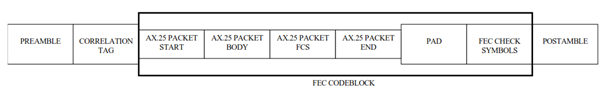
\includegraphics[width=1\textwidth]{images/fx25.png}}
\caption{FX.25 frame structure \cite{FX25}}
\label{f3.5}
\end{figure}

\newpage

\newpage
